\section{Introduction}
\label{chap:Intro}

In this note we document our measurement of the dijet mass distribution 
and our search for dijet resonances in pp Collisions at $\sqrt{s}=7$ TeV.

\subsection{History of Document}
This note is intended as documentation for a publication draft released 
under the CMS CADI heading EXO-10-010 on September 8, based on 2.875 pb$^{-1}$ of data.
A previous version of this note (AN-2010/108, V12, Archive Date August 25 2010), 
served as documentation for approved CMS results for the HCP conference on August 23, 2010,
for which the Physics Analysis Summary document is CMS PAS EXO-10-010~\cite{PAS_EXO_10-010},
based on 836 nb$^{-1}$ of data and using the eta cuts $|\Delta\eta|<1.3$ and $|\eta|<2.5$.
Another previous version of this analysis note (AN 2010/108, V11, Archive Date July 17, 2010)
was documentation for the ICHEP conference result on July 21, 2010,
for which the Physics Analysis Summary document was EXO-10-001~\cite{PAS_EXO_10-001},
based on 120 nb$^{-1}$ of data and using the single eta cut $|\eta|<1.3$ without
any cut on $\Delta\eta$. Please also see previous documents on simulation of the complete analysis
at $\sqrt{s}=10$ TeV ~\cite{CMS_AN_2009-070,CMS_AN_2009-145} and
at $\sqrt{s}=14$ TeV ~\cite{CMS_AN_2006-070}.  This analysis is synchronized
with a simultaneous analysis of the dijet centrality 
ratio~\cite{CMS_AN_2010-126} which uses the same mass bins and shared 
the data sample from the unprescaled jet trigger.

\subsection{Motivation}
Our experimental motivation is to make a first measurement of the dijet mass distribution
and see whether it agrees with expectations or contains new physics beyond the Standard Model (SM).
The LHC is a parton-parton collider in a previously
unexplored energy region. If new parton-parton resonances exist at sufficiently low mass 
then the LHC will produce 
them copiously. These resonances must also decay to partons giving two jets in the 
final state.  One theoretical motivation is that the SM has important unanswered questions.
Why do quarks come in different flavors?
Why are the quarks arranged in generations? Why are there four different forces? How do we unify gravitation with the other forces?
Why is gravity so weak? Models that try to address these questions often predict short-lived particles that
can decay to two partons: dijet resonances.

\subsection{Models}
We search for processes producing narrow resonances, $X$, decaying to dijets 
as illustrated in fig.~\ref{feyn}:
$pp \rightarrow X \rightarrow$ jet + jet (inclusive).


\begin{figure}[hbt]
  \begin{center}
      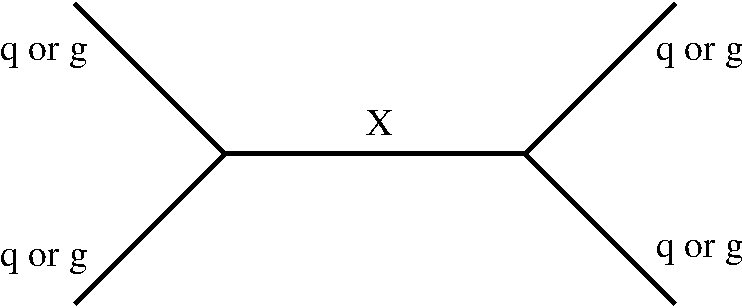
\includegraphics[width=0.5\textwidth]{Figures/resonanceDiagram.pdf}
    \caption{ Feynman Diagram of dijet resonance. The initial state and final stat
e both contain two partons (quarks, antiquarks or gluons) and the intermediate state contains 
an $s$-channel resonance $X$.}
    \label{feyn}
  \end{center}
\end{figure}


We perform a generic search that we can apply to any model.
Here we introduce some models, say a few words about the cross section, 
and explicitly list the partons involved in production and decay~\cite{CMS_AN_2006-070}. 
Excited states of 
composite quarks~\cite{Baur:1987ga} are strongly produced giving large cross sections 
($qg\rightarrow q^*$). Axigluons~\cite{Bagger:1987fz} 
or colorons~\cite{Chivukula:1996yr} 
from an additional color interaction are also strongly produced, but require an 
antiquark in the initial state ($q\bar{q} \rightarrow A$ or $C$) 
slightly reducing the cross section compared to excited quarks.  
Diquarks~\cite{Hewett:1988xc} from 
superstring inspired $E_6$ grand unified models are produced with
electromagnetic coupling from the valence quarks of the proton 
($ud \rightarrow D$). 
The cross section for $E_6$ diquarks at high mass is the largest 
of all the models considered, because at high parton momentum the 
probability of finding a quark 
in the proton is significantly larger than the probability of finding a 
gluon or antiquark. 
Randall Sundrum gravitons~\cite{RS}, with coupling $k/M_{PL}=0.1$, from a model of 
large extra dimensions are produced 
from gluons or quark-antiquark pairs in the initial state ($q\bar{q},gg \rightarrow G$).
Heavy $W$ bosons~\cite{Eichten:1984eu} inspired by left-right
symmetric grand unified models have electroweak couplings 
and require antiquarks for their
production($q_1 \bar{q_2} \rightarrow W^{\prime}$), giving small cross sections.  
Heavy $Z$ bosons~\cite{Eichten:1984eu} 
inspired by grand-unified models are widely anticipated by theorists, 
but they are electroweakly produced, 
and require an antiquark in the initial state($q\bar{q} \rightarrow Z^{\prime}$), 
so their production cross section is around the lowest of the models considered.
The model with the largest cross section is a recent model of string resonances, 
Regge excitations of the quarks and gluons in open string theory, which
includes resonances in three parton-parton channels (predominantly $qg$ at LHC but also some $q\bar{q}$ and $gg$)
with multiple spin states and quantum numbers~\cite{Anchordoqui:2008di,Cullen:2000ef}.
Table~\ref{table:models} summarizes some properties of these models, and the string resonance model
is discused in detail in Appendix~\ref{appString}.


\begin{table}[th]
\centering
\normalsize
       \begin{tabular}{|c|c|c|c|c|c|}
        \hline
        Model Name 	& X & Color 	& $J^{P}$ 	& $\Gamma /(2M)$ & Chan		\\
        \hline
	Excited Quark 	& q*& Triplet 	& $1/2^+$ 	& $0.02$ 	& qg		\\
        E$_{6}$ Diquark & D & Triplet 	& $0^+$ 	& $0.004$ 	& qq		\\
        Axigluon 	& A & Octet 	& $1^+$ 	& $0.05$ 	& $q\bar{q}$	\\
        Coloron 	& C & Octet 	& $1^-$ 	& $0.05$ 	& $q\bar{q}$	\\
        RS Graviton 	& G & Singlet 	& $2^+$ 	& $0.01$ 	& $q\bar{q}$ , gg	\\
        Heavy W 	& W'& Singlet 	& $1^-$ 	& $0.01$ 	& $q\bar{q}$	\\
        Heavy Z 	& Z'& Singlet 	& $1^-$ 	& $0.01$ 	& $q\bar{q}$	\\
	String          & S & mixed     & mixed         & $0.003-0.037$  & $qg$, $q\bar{q}$, $gg$ \\
        \hline
        \end{tabular}
 	\caption{Properties of Some Resonance Models}
	\label{table:models}
	\end{table}



Published lower limits~\cite{Aaltonen:2008dn} on the mass of these models in the dijet channel are 
listed in table~\ref{tab:tevatronLimits}.
\begin{table}[tbh]
\begin{center}
\begin{tabular}{|c|c|c|c|c|c|c|c|}\hline
 $q^*$ & $A$ or $C$ & $D$  & $\rho_{T8}$ & $W^{\prime}$ & $Z^{\prime}$ & $G$ &
 $S$\\ \hline
 1.26  & 1.25       & 0.63 &  1.1       &  0.84         &   0.74       & - & 1.4$^*$\\ \hline
\end{tabular}
\caption[]{ Published lower limits in dijet channel in TeV on the mass of new particles considered in this
analysis.  These 95\% confidence level exclusions are from the Tevatron~\cite{Aaltonen:2008dn}, except
for the $q^*$ limit which is from ATLAS~\cite{ATLAS_Search}.
The string resonance mass limit comes from the cross section upper limit at the Tevatron and our 
evaluation of the string resonance cross section as shown in Fig.~\ref{CDFstringLimit}.}
\label{tab:tevatronLimits}
\end{center}
\end{table}


\subsection{Summary of Experimental Technique}
Our experimental technique starts with a measurement of the 
inclusive process $pp \rightarrow$ jet + jet + anything.  Inclusive means we
measure processes containing at least two jets in the final state, but the 
events are allowed to contain additional jets, or anything else.
The dijet in the event is simply the two highest pt jets, the leading jets.
Within the standard model our dataset is expected to be overwhelming
dominated by the $2\rightarrow 2$ process of hard parton scatters, with 
additional radiation off the initial
and final state partons naturally giving additional jets. We do not cut
away events that contain this radiation, which would reduce signals that 
also have similar amounts of radiation, 
and un-necessarily restrict signals to a narrow topology.  The 
events can also contain additional particles, such as leptons or photons, 
but this will occur very rarely in the standard model.  Finally, even more
rarely within the standard model, the two leading CaloJets in the event can
result from electrons, photons or taus producing energy in the calorimeter,
and we do not exclude these insignificant contributions to our sample either.  
Our dijet selection is then open to many signals of new physics including 
high pt jets, leptons and photons. However, our selection is optimized for 
signals in the $2\rightarrow 2$ parton scattering process, and is
overwhelmingly dominated by the signal background of dijets from QCD within 
the standard model.


Our experimental method to search for dijet resonances utilizes 
the dijet mass spectrum measured from the two leading jets in the data.  
If a dijet resonance exists, it should appear in the dijet mass spectrum 
as a bump. First we compare the dijet mass spectrum to QCD predictions 
from PYTHIA to see if they agree, but we do not use QCD to model our 
background in the search.  We use a smooth parameterization to model our 
background. We fit the dijet mass spectrum with a smooth parameterization 
and see whether we can get a good fit.  The fit probability tells us whether
the data is smooth, which is the first test for the presence of a resonance.
We look at the difference between the data and the fit, and estimate the 
significance of  the largest upward fluctuation in the data interpreted as 
a narrow resonance.  If there is no significant evidence for dijet resonances, 
we proceed to set limits. The dijet resonance shape for generic di-parton 
resonances containing qq, qg and gg partons were simulated using PYTHIA as 
resonance signals. To calculate the upper cross section limit for this dijet 
resonance shape in our data, we use a binned maximum likelihood method. The 
method gives a Poisson likelihood as a function of the cross section. 
We convolute the statistical likelihood distribution with our Gaussian 
systematic uncertainty and find the 95\% confidence
level upper limit on the cross section. This gives cross section limits for 
generic narrow qq, qg and gg resonances, independent of any specific resonance 
model.  The upper limit on the cross section is then compared with the 
predicted cross section for a few benchmark models to obtain mass limits on 
particular models. This experimental method is basically the same as 
that employed by the dijet resonance searches at the 
Tevatron~\cite{Aaltonen:2008dn,Abazov:2003tj,Abe:1997hm} and at 
ATLAS~\cite{ATLAS_Search}.
